% Тут используется класс, установленный на сервере Papeeria. На случай, если
% текст понадобится редактировать где-то в другом месте, рядом лежит файл matmex-diploma-custom.cls
% который в момент своего создания был идентичен классу, установленному на сервере.
% Для того, чтобы им воспользоваться, замените matmex-diploma на matmex-diploma-custom
% Если вы работаете исключительно в Papeeria то мы настоятельно рекомендуем пользоваться
% классом matmex-diploma, поскольку он будет автоматически обновляться по мере внесения корректив
%

% По умолчанию используется шрифт 14 размера. Если нужен 12-й шрифт, уберите опцию [14pt]
% \documentclass[14pt]{matmex-diploma}
\documentclass[14pt]{matmex-diploma-custom}

\begin{document}
% Год, город, название университета и факультета предопределены,
% но можно и поменять.
% Если англоязычная титульная страница не нужна, то ее можно просто удалить.
\filltitle{ru}{
    chair              = {Программная инженерия\\Кафедра системного программирования},
    title              = {Разработка системы предсказания вторичной структуры РНК с использованием синтаксического анализа и искусственных нейронных сетей},
    % Здесь указывается тип работы. Возможные значения:
    %   coursework - Курсовая работа
    %   diploma - Диплом специалиста
    %   master - Диплом магистра
    %   bachelor - Диплом бакалавра
    type               = {coursework},
    position           = {студента},
    group              = 371,
    author             = {Кутленков Дмитрий Александрович},
    supervisorPosition = {к.\,ф.-м.\,н., доцент},
    supervisor         = {Григорьев С.\,В.},
    reviewerPosition   = {},
    reviewer           = {},
    chairHeadPosition  = {},
    chairHead          = {},
%   university         = {Санкт-Петербургский Государственный Университет},
%   faculty            = {Математико-механический факультет},
%   city               = {Санкт-Петербург},
%   year               = {2013}
}
%\filltitle{en}{
%    chair              = {The Meaning of Life \\ Uselessness of Everything},
%    title              = {Empty subset as closed set},
%    author             = {Edelweis Mashkin},
%    supervisorPosition = {professor},
%    supervisor         = {Amvrosy Vibegallo},
%    reviewerPosition   = {assistant},
%    reviewer           = {Alexander Privalov},
%    chairHeadPosition  = {professor},
%    chairHead          = {Christobal Junta},
%}
\maketitle
\tableofcontents
% У введения нет номера главы
\section*{Введение}
Многие направления современной биоинформатики имеют дело с анализом биологических последовательностей. Наиболее интересным объектом для изучения являются кодирующие последовательности, присутствующие в клетках всех живых организмах --- РНК и ДНК. \par
РНК --- макромолекула, выполняющая множество различных функций в живых организмах. РНК состоит из цепи нуклеотидов --- базовых органических соединений, с помощью которых в организме кодируется информация. Таким образом, РНК является носителем генетических функций и выполняет работу по переносу и реализации этой информации, например, играет основную роль в процессе синтеза белков --- трансляции. Однако ее функции не ограничиваются трансляцией --- она играет важную роль во множестве других процессов~\cite{book:molcelbio}. \par
Как и другие макромолекулы, РНК практически никогда не находится в развернутом виде --- она некоторым образом сворачивается в пространстве. При рассмотрении структур макромолекул выделяют несколько уровней (см. Рис.~\ref{fig:Структура}). Для понимания функций РНК зачастую необходимо знать ее структуру~\cite{SARAIYA2008645, LEE1997732}. Предсказывать вторичную структуру РНК проще, чем третичную, к тому же она предоставляет информацию, полезную для предсказания третичной структуры~\cite{ipknot}. Экспериментальные методы предсказания вторичной структуры (такие, как ядерный магнитный резонанс и рентгеноструктурный анализ) сложны и требуют большого количества ресурсов. Из-за этого предпочитаемыми способами предсказания являются вычислительные методы. \par 
При построении цепи РНК используются 4 нуклеотида. Они являются парными, то есть могут образовывать между собой связи. Вторичная структура РНК описывает водородные связи между нуклеотидами. Она может включать в себя несколько базовых структурных элементов, одним из самых частых является "шпилька" (см. Stem loop на Рис.~\ref{fig:Структура}) --- элемент, состоящий из нескольких последовательно связанных нуклеотидов, за которыми идут несколько не связанных. \par 
\begin{figure}[h]
	\centering
	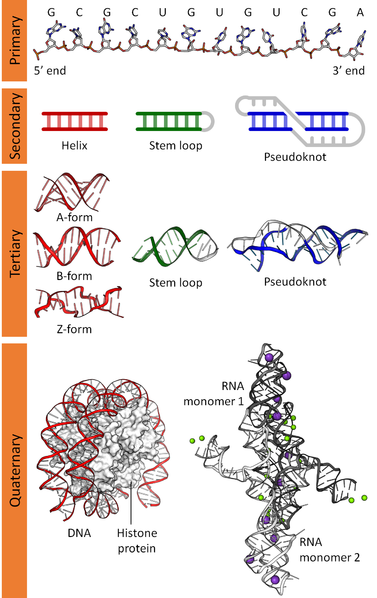
\includegraphics{pics/DNA_RNA_structure_(full).png}
	\caption{Структура РНК~\cite{Wikipediapic}}
	\label{fig:Структура}
\end{figure}
Когда мы говорим о вторичной структуре РНК, нужно помнить о том, что в ней возможны псевдоузлы --- структурные элементы, в которых новая "шпилька" начинается в момент, когда предыдущая еще не закончилась (см. Pseudoknot на Рис.~\ref{fig:Структура}). Этот элемент накладывает ограничения на методы, которые мы можем использовать при предсказании вторичной структуры, и делает неприменимыми некоторые классические решения. В связи с этим на данный момент лишь относительно небольшое количество инструментов(см.~\hyperref[obzor]{Обзор существующих решений}) предсказания вторичной структуры позволяют предсказывать псевдоузлы. Поэтому создание инструмента, умеющего учитывать псевдоузлы, было одним из направлений нашего проекта.

\section{Постановка задачи}
Целью данной работы является разработка системы, способной с достаточной степенью точности предсказывать вторичную структуру РНК, учитывая при этом псевдоузлы. \par 
Для достижения цели были поставлены следующие задачи:
\begin{itemize}
	\item Изучить предметную область
	\item Проанализировать существующие решения
	\item Спроектировать систему на основе формальных грамматик и нейронных сетей
	\item Собрать и обработать данные для обучения нейронной сети
%	\item Выбрать для использования наиболее подходящие реализации парсера и нейронной сети. Поставить на них эксперименты и проанализировать их результаты, внося изменения в систему при необходимости
	\item Создать систему для подготовки данных
	\item Обработать результат нейронной сети для получения биологически возможного результата
	\item Собрать составные части в единую систему, с которой будет удобно работать целевой аудитории, то есть биологам и биоинформатикам
\end{itemize}
\section{Обзор существующих решений}
\subsection{Обзор существующих методов}\label{obzor}
Существующие вычислительные методы можно разделить на две категории --- проводящие сравнительный анализ и проводящие анализ одной последовательности. В своем обзоре я не буду касаться первого вида, так как он составляет вторичную структуру основываясь на нескольких гомологичных входных последовательностях, и сосредоточусь на обзоре решений, работающих непосредственно с одной цепочкой.  \par 
Одним из популярных подходов для предсказания вторичной структуры является нахождение структуры с минимальной свободной энергией (MFE метод). Такие инструменты используют динамический подход --- считают энергию конечной структуры, основываясь на энергиях составных частей. В качестве примера такого подхода можно привести {\it RNAfold}~\cite{Hofacker1994}. Другой подход, увеличивающий точность MFE методов --- метод максимальной ожидаемой точности (MEA метод), который выбирает наиболее точную структуру из возможных. Примером такого метода является {\it CentroidFold}~\cite{hamadaCentroid}. \par
Однако же, у перечисленных выше методов есть существенный недостаток --- они не умеют предсказывать псевдоузлы, которые играют важную роль как в клетках, так и в вирусах~\cite{StaplePseudo, DEIMAN1997166}. \par
Для предсказания структур с псевдоузлами существует ряд других методов. {\it HotKnots}~\cite{Hotknots} использует схожий с MFE метод, добавляя части структуры в попытке минимизировать общую энергию структуры. Это, однако, занимает большое количество времени. Расширением MEA метода является {\it IPknot}~\cite{ipknot} --- метод, использующий целочисленное программирование для приближения распределения вероятностей связей между нуклеотидами в последовательности. Еще одним методом, основывающимся на гипотезе о том, что цепочки сначала складываются в структуры без псевдоузлов, а потом проводят дополнительные связи для минимизации энергии~\cite{TINOCO1999271}, является {\it HFold}~\cite{Hfold}. Позднее была выпущенная улучшенная версия --- {\it Iterative HFold}~\cite{ihfold}, которая исправила проблемы, связанные с псевдоузлами. Тесты представленных программ, однако, не позволяют говорить об однозначном превосходстве какой-либо из них~\cite{comparision}. \par 
Стоит отметить, что структуру РНК без псевдоузлов можно задать с помощью контекстно-свободной грамматики~\cite{rnacf}. Также доказано, что можно задать вторичную структуру, используя стохастические контекстно-свободные грамматики~\cite{Knudsen1999RNASS}. Однако, в общем случае создание и применение такой грамматики слишком сложная задача, так как в природе при определенных условиях существует вероятность создания нетипичных соединений. Поэтому на практике предполагается использовать формальные грамматики для получения базовой структуры, а сложные взаимодействия обрабатывать с применением другого метода. \par 
При работе с реальными данными нужно иметь в виду, что они подвержены большому числу искажений, возникающих как из-за технических причин (ошибки при получении данных с макромолекулы), так и из-за биологических (мутации). Это делает плохо применимыми точные методы. Одним из способов борьбы с этой проблемой является использование методов машинного обучения, например, искусственных нейронных сетей. Недавние успехи в области предсказания структуры белков с помощью нейронных сетей позволяют рассматривать этот метод как потенциально успешный в области предсказания структуры РНК~\cite{Wang073239}. Кроме того, на данный момент существует несколько проектов, ведущих исследования по предсказанию структуры РНК с помощью методов машинного обучения, например, LSTM сетей~\cite{lstmnetwork} и ансамблей сетей~\cite{ensemblenetwork}.\par  
Комбинируя методы синтаксического анализа и машинного обучения, то есть извлекая основные особенности структуры с помощью алгоритмов синтаксического анализа, а затем обрабатывая полученные данные с помощью нейронной сети, мы хотим получить систему, способную достаточно точно предсказывать вторичную структуру РНК с учетом псевдоузлов. Так как работа была выполнена в рамках исследовательского проекта с несколькими участниками, был использован уже готовый парсер, а нейронная сеть разрабатывалась параллельно с данной работой магистранткой кафедры системного программирования Полиной Сергеевной Луниной. Опишем эти составные части подробнее.
\subsection{Парсер}
Парсер принимает на вход первичную структуру (строку, в которой записана последовательность нуклеотидов) и распознает возможные места для соединений между нуклеотидами. На выходе парсер выдает картинку, в которой белые пиксели стоят в позиции $[i,j]$, если между $i$-м и $j$-м нуклеотидом возможна связь. На диагонали в картинке стоят пиксели различного цвета в зависимости от нуклеотида --- это необходимо для того, чтобы была возможность восстановить изначальную структуру. Парсер создан с помощью платформы {\it YaccConstructor}~\cite{yacc}.
\begin{figure}[h]
	\centering
	\captionsetup{justification=centering}
	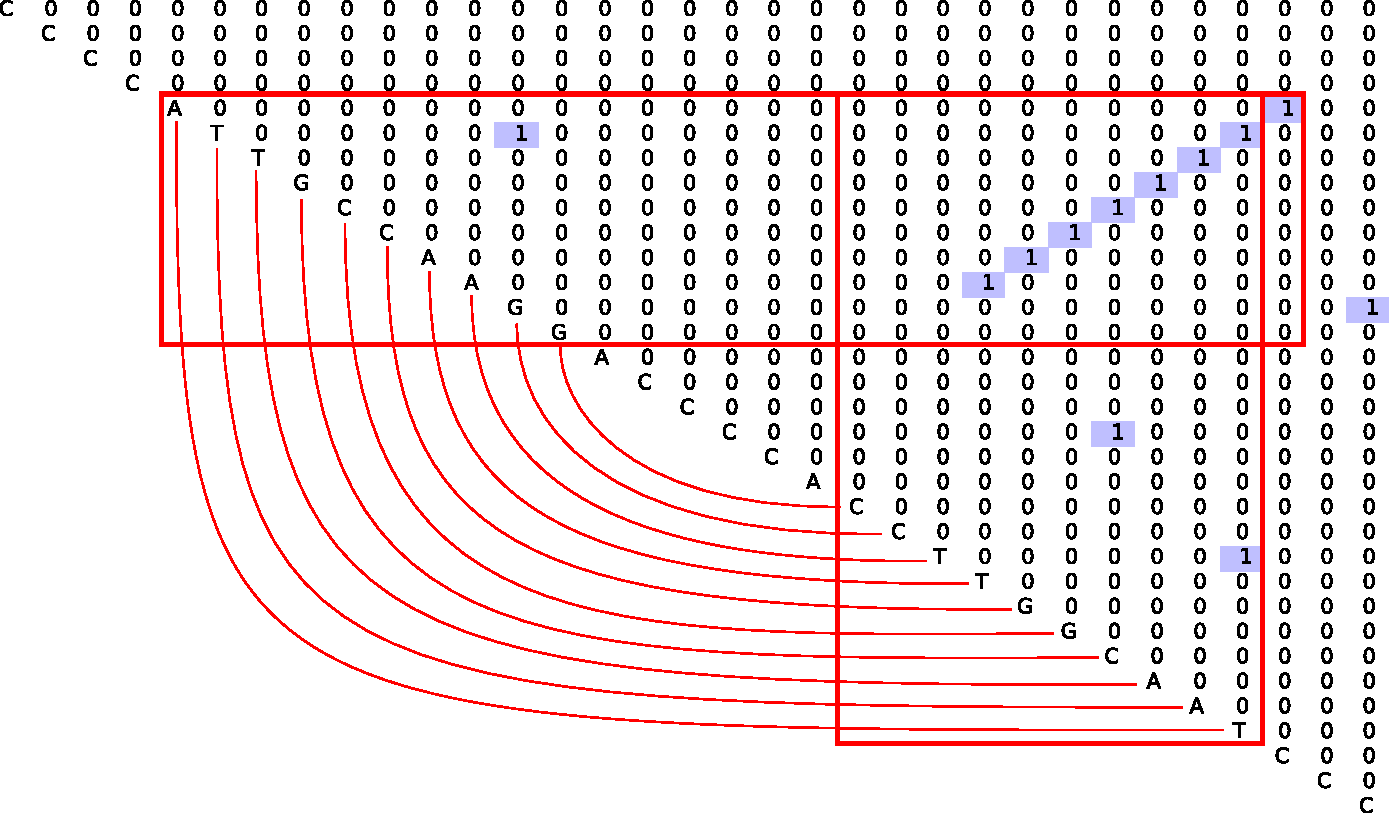
\includegraphics[scale=0.6]{pics/4.pdf}
	\caption{Представление вторичной структуры, используемое в работе (для последовательности ДНК)~\cite{semyonandpolina}}
	\label{fig:Структура}
\end{figure}
\subsection{Нейронная сеть}
Нейронная сеть должна уметь очищать результат работы парсера от ненужных связей. Для обучения нейросети мы подаем ей на вход результат работы парсера и эталонную структуру в виде картинки. Нейросеть должна быть способна предсказывать сложные связи внутри структуры и взаимодействия между базовыми структурами. На данный момент используется остаточная нейронная сеть. \par
Так как итоги работы над нейронными сетями важны для понимания работы в целом, кратко приведем полученные результаты. \par
Предпринимались попытки использования двух подходов к созданию нейросети c использованием данных, подготовленных в рамках этой курсовой работы. Первый заключался в том, чтобы использовать данные примерно одинаковой длины и дополнять более короткие последовательности до самой длинной, заполняя недостающую часть изображения черными точками. Другой позволял использовать данные разной длины.
\subsubsection{Сеть для данных фиксированной длины}
При обучении данной сети были использованы 56689 последовательностей длиной 90 нуклеотидов, разделенных на обучающую, валидационную и тестовую выборки в отношении 70\%:10\%:20\%. Наилучший полученный результат имеет F-меру (среднее гармоническое precision и recall) равную 87\%.
\subsubsection{Сеть для данных переменной длины}
Реальные последовательности имеют разную длину, поэтому была использована другая архитектура, позволяющая обучаться на данных переменной длины. Кроме того, такая архитектура позволяет нам использовать больше данных. Были использованы 145054 цепочек длиной от 50 до 90 нуклеотидов, разделенных в той же пропорции.
Для этих данных удалось достичь значения F-меры равного 62\%. \par 
Полученную сеть дообучили на данных с псевдоузлами. F-мера нейросети поднялась до 75\%. Провести тестирование по качеству предсказания исключительно псевдоузлов пока не удалось, но полученные результаты показывают потенциал дальнейших исследований в данном направлении.
\par Полученные результаты имеют один существенный недостаток --- используемые методы обучения и измерения качества нейронной сети плохо отслеживают, между какими из нуклеотидов устанавливаются связи, в то время как на самом деле в подавляющем большинстве случаев связи образуются между парными нуклеотидами. Этот факт породил необходимость использовать алгоритм выравнивания, о котором будет рассказано далее.
\section{Архитектура процесса обучения \\ нейронной сети}
Для выполнения поставленной задачи была разработана следующая архитектура (Рис.~\ref{fig:process}). Рассмотрим общий процесс работы системы. \par
\begin{figure}[h]
\centering
\begin{tikzpicture}[node distance=1cm, auto]  
\tikzset{
	mynode/.style={rectangle,rounded corners,draw=black, top color=white, bottom color=yellow!50,very thick, inner sep=1em, minimum size=3em, text centered},
	myarrow/.style={->, >=latex', shorten >=1pt, thick},
	mylabel/.style={text width=7em, text centered} 
}  
\node[mynode] (base) {База вторичных структур};  
\node[below=4cm of base] (dummy) {}; 
\node[mynode, left=of dummy] (parser) {Парсер};  
\node[mynode, right=of dummy, align = center] (script) {Скрипт преобразования \\ вторичной структуры};
\node[mylabel, below left=of base] (label1) {Первичная структура};  
\node[mylabel, below right=of base] (label2) {Вторичная структура};
% The text width of 7em forces the text to break into two lines. 

\draw[myarrow] (base.south) -- ++(-.5,0) -- ++(0,-1) -|  (parser.north);	
\draw[myarrow] (base.south) -- ++(.5,0) -- ++(0,-1) -|  (script.north);
% There is a slight overlap of the arrows with the (manufacturer) south edge
% because creating the offset in another way didn't compile. 
\node[mynode, below=4cm of dummy] (neuro) {Нейронная сеть}; 
\draw[myarrow] (parser.south) -- ++(0,-1) -|  (neuro.north);
\draw[myarrow, rotate = 90] (script.south) -|  (neuro.east);
\node[mylabel, below =of script, xshift = 15mm] (label2) {png файл};
\node[mylabel, below =of parser, xshift = -15mm] (label2) {png файл};
%\draw[<->, >=latex', shorten >=2pt, shorten <=2pt, bend right=45, thick, dashed] 
%(retailer1.south) to node[auto, swap] {Competition}(retailer2.south); 
% The swap command corrects the placement of the text.

\end{tikzpicture} 
\medskip
\caption{Архитектура процесса обучения нейронной сети} 
\label{fig:process}
\end{figure}
В процессе обучения нейросети из базы берутся пары из первичной (строка, в которой записана последовательность нуклеотидов) и вторичной (строка в формате dot-bracket --- в ней непарные нуклеотиды отмечены точками, а парные отмечаются парными скобками) структур последовательности. Первичная структура отправляется на вход парсера, а вторичная на вход скрипта, который превращает ее в изображение, где белые пиксели стоят в позиции $[i,j]$, если между $i$-м и $j$-м нуклеотидом есть связь. Выход парсера и скрипта мы передаем на вход нейронной сети. Таким образом, сеть учится убирать ненужные связи и добавлять недостающие в результат работы парсера. \par
Используемые парсер и нейросеть были описаны ранее. Рассмотрим оставшийся компонент --- данные.
\subsection{Данные}
В качестве данных для обучения нейросети мы используем пары из последовательности нуклеотидов и ее вторичной структуры. Наилучшим вариантом является использование данных, полученных биологическими методами. Баз с такими последовательностями существует две --- {\it RNA STRAND}~\cite{rnastrand} и {\it Pseudobase++}~\cite{pseudobase}. К сожалению, в этих базах довольно мало данных. Для обучения нейросети требуется много данных примерно одинаковой длины. В результате было решено использовать последовательности из базы РНК {\it RNAcentral}~\cite{rnacentral}, а затем получать их вторичные структуры с помощью сторонних инструментов. После получения хорошего результата для последовательностей без псевдоузлов можно использовать дообучение нейронной сети на данных с псевдоузлами.

\section{Архитектура конечной системы}
Итоговая система была воплощена в виде веб-сервиса. Серверная часть написана на языке \textit{Python 3}, с использованием библиотеки \textit{flask}\footnote{Фреймворк для создания веб-приложений на языке Python: \url{https://palletsprojects.com/p/flask/}[Accessed: 15th April, 2020].}. Общение между клиентом и сервером происходит с помощью \textit{REST API}. Клиентская часть написана с помощью фреймворков \textit{Vue.js}\footnote{JavaScript-фреймворк для создания пользовательских интерфейсов: \url{https://vuejs.org/}[Accessed: 15th April, 2020].} и \textit{Bulma.io}\footnote{CSS-фреймворк: \url{https://bulma.io/}[Accessed: 15th April, 2020].}. Вышеперечисленные технологии были выбраны, так как они позволяют в сжатые сроки создать прототип, который затем будет удобно расширять. \par
\begin{center}
	\hspace*{-5cm}%
	\begin{tikzpicture}[node distance=1cm, auto, title/.style={font=\fontsize{6}{6}\color{black!50}\ttfamily}]  
	\tikzset{
		mynode/.style={rectangle,rounded corners,draw=black, top color=white, bottom color=yellow!50,very thick, inner sep=1em, minimum size=3em, text centered},
		myarrow/.style={->, >=latex', shorten >=1pt, thick},
		mylabel/.style={text width=7em, text centered} 
	}  
    \node (decomp) [title, minimum height = 30pt, minimum width =230pt, label={[anchor=north west, inner sep=0pt]north west: Клиент} ] { };
    \node[below right=of decomp] (dummy) {}; 
    
	\node[mynode, left =of dummy] (base) {Входная последовательность}; 
	\node[mynode, right=of dummy] (result) {Результат}; 
	\node [draw=black!50, fit={(decomp) (base) (result)}] {}; 
	
	\node (server) [minimum height = 30pt, minimum width =220pt,below=of base, label={[anchor=north west, inner sep=0pt]north west: Сервер}] {  };
	\node[mynode, below=of server] (parser) {Парсер};
	\node[mynode, below=of parser] (network) {Нейронная сеть};
	\node[mynode, below=of network] (converter) {Преобразователь в строку};
	\node[mynode, below=of converter] (aligner) {Выравниватель};
	\node [draw=black!50, fit={(server) (parser) (network) (aligner) (converter)}] {};
	\node[mylabel, below left=of base] (label1) {};  
	\node[mylabel, below right=of base] (label2) {};
	% The text width of 7em forces the text to break into two lines. 
	
	\draw[myarrow] (base.south)  -|  (parser.north);
	% There is a slight overlap of the arrows with the (manufacturer) south edge
	% because creating the offset in another way didn't compile. 
	\draw[myarrow] (parser.south)  -|  (network.north);
	\draw[myarrow] (network.south)  -|  (converter.north);
	\draw[myarrow] (converter.south)  -|  (aligner.north);
	\draw[myarrow] (network.east)  -|  (result.south);
	\draw[myarrow] (converter.east)  -|  (result.south);
	\draw[myarrow] (aligner.east)  -|  (result.south);
	%\draw[<->, >=latex', shorten >=2pt, shorten <=2pt, bend right=45, thick, dashed] 
	%(retailer1.south) to node[auto, swap] {Competition}(retailer2.south); 
	% The swap command corrects the placement of the text.
	
	\end{tikzpicture} 
\end{center} \par
Парсер и нейронная сеть были рассмотрены ранее. Рассмотрим подробнее алгоритм выравнивания.
\subsection{Алгоритм выравнивания}
Нейронная сеть плохо способна отслеживать, между какими из нуклеотидов она предсказывает связи. Так как в основном в природе связи образуются между парными нуклеотидами, необходимо обработать результат. Для этого был разработан алгоритм, в основе которого лежит следующая идея --- если в предсказанной нейросетью последовательности существует какая-то петля, то где-то рядом с этим местом энергетически выгодно образовать петлю схожего размера. Алгоритм состоит из следующих шагов:
\begin{enumerate}
	\item Найти следующую петлю
	\item Расширить границы, в которых мы будем искать выравнивание. Важно не пересекать петли между собой.
	\item На полученных интервалах провести локальное выравнивание
	\item Запомнить границы найденного результата
	\item Вернуться в п. 1
\end{enumerate}
% У заключения нет номера главы
\section*{Заключение}
В рамках курсовой работы были выполнены следующие задачи:
\begin{itemize}
	\item Изучена предметная область
	\item Проведен анализ уже существующих решений
	\item Разработана архитектура системы
	\item Собраны, проанализированы и  обработаны данные из нескольких источников - \textit{RNA STRAND}, \textit{Pseudobase++}, \textit{RNACentral}
%	\item Проведены эксперименты с различными данными и подходами к архитектуре нейронной сети. В качестве основы использована остаточная нейронная сеть.
	\item Создана система подготовки данных
	\item Разработан алгоритм перевода полученных последовательностей в биологически возможные
	\item Разработана система предсказания вторичной структуры РНК последовательностей
	\item Создано клиент-серверное приложение, предоставляющее доступ к системе
\end{itemize} \par
Исходный код доступен по ссылкам \url{https://github.com/SacredArrow/Secondary_structure_public} и \url{https://github.com/SacredArrow/Course_work_web}.\par 
Разработанная система задумывалась максимально простой для пользователя и поэтому может быть использована биологами и биоинформатиками при проведении исследований. \par 
Данная система может быть улучшена путем улучшения составных систем, например, нейронной сети. Улучшение может состоять как в получении дополнительных данных, так и в дальнейших экспериментах с архитектурой. Также для системы удалось лишь частично поддержать псевдоузлы, так как они требуют более сложной постобработки.


\setmonofont[Mapping=tex-text]{CMU Typewriter Text}
% \bibliographystyle{ugost2008ls}
\bibliographystyle{ieeetr}
\bibliography{diploma.bib}
\end{document}
